%----------------------------------------
% Write your notes here
%---------------------------------------
\setlength{\parindent}{4em}
\setlength{\parskip}{1em}
\renewcommand{\baselinestretch}{1}
 
\textbf{NOTES}

\textbf{1.Computational Tractability} 
\begin{itemize}
\item 
The optimal value could be calculated in a reasonable amount of time.
\end{itemize}

\textbf{2.Asymptotic order of growth --- Big O notation}
\begin{itemize}
\item
It is used to understand approximation when variables go to infinite. 
\item
In computer science, big O notation is usually used to evaluate algorithms on their running time and space as the input size grows.
\end{itemize}

\textbf{3.Common running times} 
\begin{itemize}
\item 
It depends on data structure and algorithms.
\end{itemize}

\textbf{4.Running time in size n input}
\begin{itemize}
\item 
brute force algorithm : $2^{n}$ $\Rightarrow$ exponential 
\item
$c n^{d}$ ($c>0$ $d>0$) $\Rightarrow$ polynomial
\item
It is theoretical step here, but does not perform well in practice purpose. \\ 
Constant matter: $\underbrace{20 n^{100}}_{polynomial}$ vs $\underbrace{n^{1+0.02 lgn}}_{not polynominal, but still better}$ $\Rightarrow$ So notice that constant cannot be ignored! \\
\item
Order of running time: $n<nlogn<n^{2}<n^{3}<1.5 n^{3}<2^{n}<n!$
\end{itemize}



\textbf{5.Runtime analysis}
\begin{enumerate}
\item 
Worst-case Complexity analysis(Our focus):\\
Worst-case Complexity analysis considers the maximal complexity of the algorithm over all possible inputs.
\item
Average-case Complexity: \\
Average-case Complexity considers the average complexity over all possible inputs. (Making an assumption of the statical distribution of the inputs $\Rightarrow$ expected time, uniform distribution) It may be a more accurate measure of an algorithm's performance in practice. 
\item
Amortized Analysis:\\
Amortized Analysis considers the running time for a sequence of operations rather than worst-case analysis focusing on each operation. \\

- Eg. In stack, we push in for O(1), pop all for O(n) in worst case.\\
For worst-case analysis, its running time should be O(n);\\
For average-case analysis, calculate the expectation of it; \\
For amortized analysis, O(1). 
\end{enumerate}


\textbf{6.Asymptotic Analysis}
\begin{enumerate}
\item 
- Upper Bound(Big-O notation):\\
For a function T(n)(running time of y), f(n) is an upper bound if for "big enough n", $\exists c >0 $, $T(n) \leq cf(n)$. Here f dominates T.(Figure1)\\
\begin{figure}
\centering
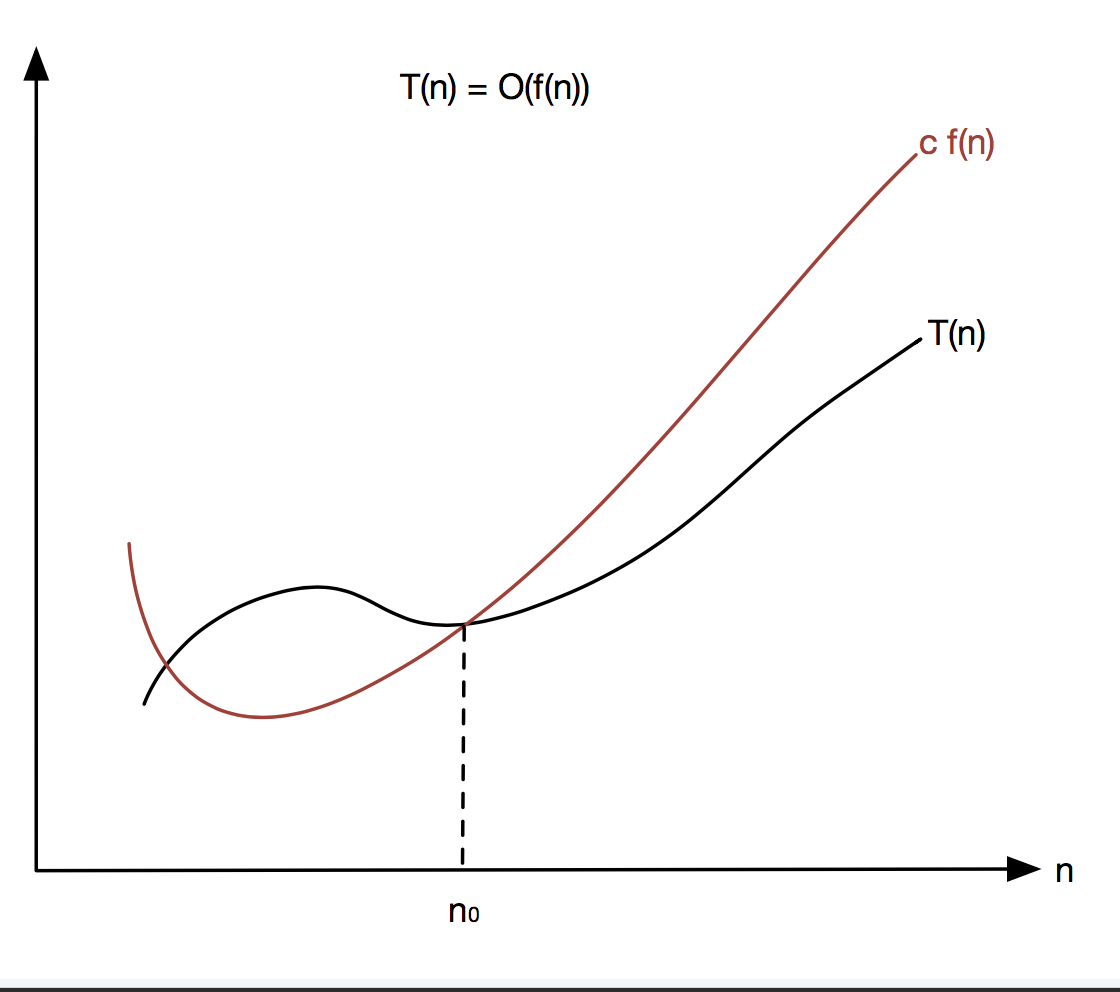
\includegraphics[width=0.3\textwidth]{big-O.png}
\caption{\label{fig:big-O}Big-) notation}
\end{figure}
Eg. $T(n) = 32 n^{2} + 17n + 1$ $\Rightarrow$ $T(n) = O(n^{2})$, choose $ c=50, n= 1$ 
\item
- Lower Bound(Big-$\Omega$ notation):\\
For a function T(n)(running time of y), f(n) is a lower bound if for "big enough n", $\exists c >0 $, $T(n) \leq cf(n)$. Here f dominates g. (Figure2)\\
\begin{figure}
\centering
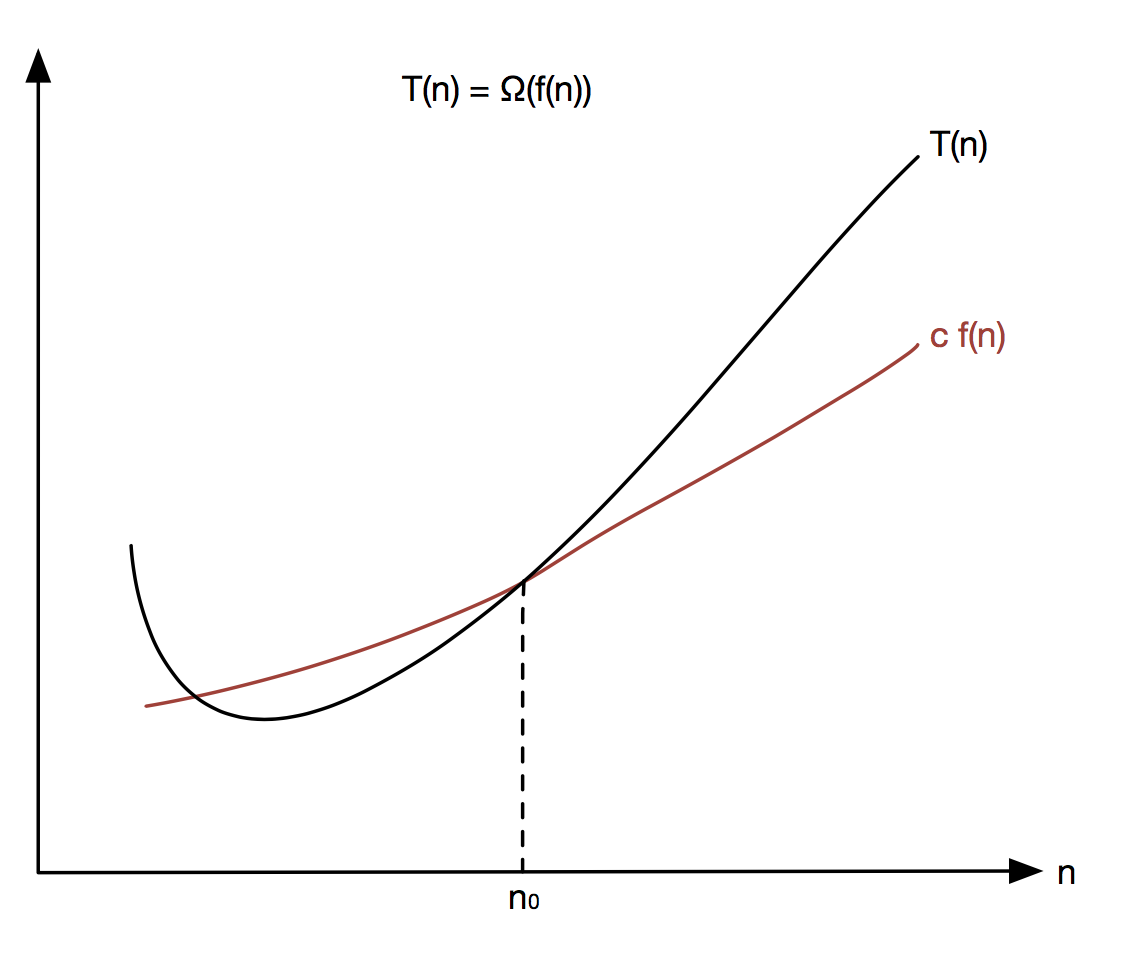
\includegraphics[width=0.3\textwidth]{big-Omega.png}
\caption{\label{fig:big-Omega}Big-Omega notation}
\end{figure}
Eg. For the same example $\Rightarrow$ $T(n)= \Omega(n)$; $T(n)= \Omega(n^{2})$, choose $c = 31, n \geq 1$ 
\item
-Tight Bound(Big-$\Theta$ notation):\\
If f(n) is both upper bound and lower bound of T(n) [with different c], we say f(n) is a tight bound for T(n). That is, $\exists c_{1} >0, c_{2}>0$, $ c_{1} f(n) \leq T(n) \leq c_{2}f(n)$.(Figure3)\\
\begin{figure}
\centering
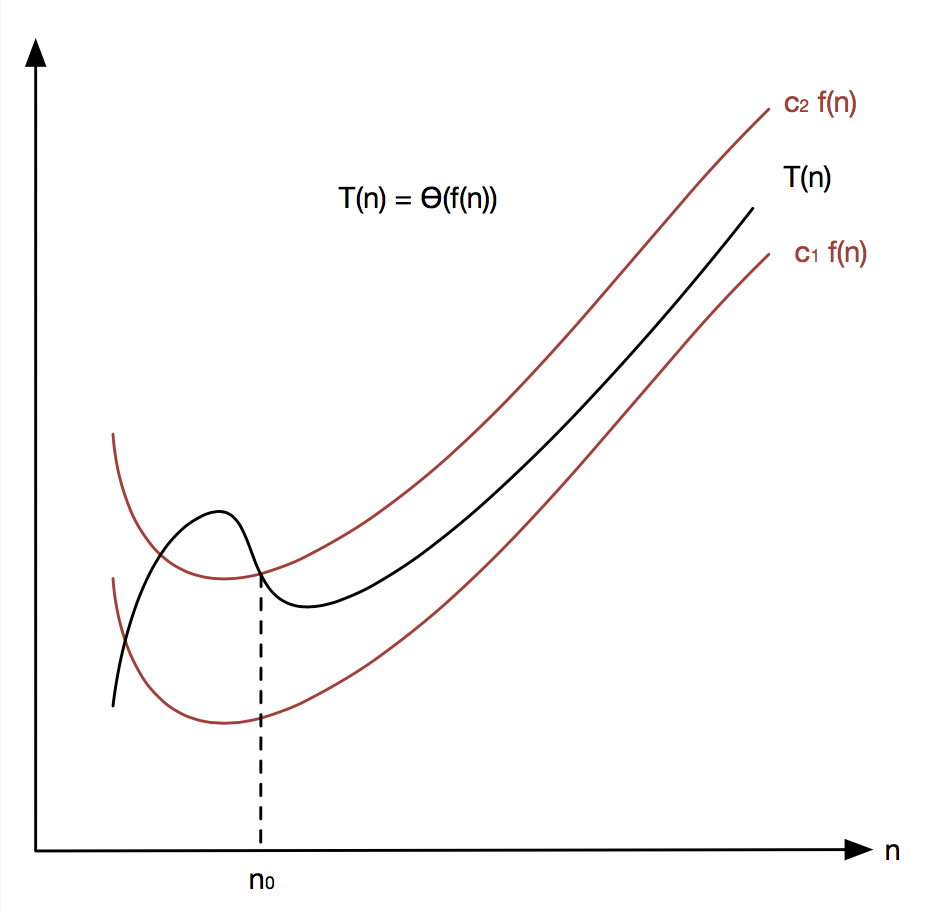
\includegraphics[width=0.3\textwidth]{big-theta.png}
\caption{\label{fig:big-theta}Big-Theta notation}
\end{figure}
Eg. For the same example $\Rightarrow$ $T(n)= \Theta(n^{2})$
\end{enumerate}

\pagebreak
\textbf{7. Rules of Thumb} 
\begin{enumerate}
\item 
$T(n) = a_{0} + a_{1}n + \dots + a_{d}n^{d}$ $\Rightarrow$ $T(n) = O(n^{d})$
\item
$O(log_{a}^{n}) = O(log_{b}^{n})$,  $a, b>0$ 
\item
For every $r>1, d>0$ $\Rightarrow$ $n^{d} = O(r^{n})$ 
\end{enumerate}

\textbf{8. Examples}
\begin{enumerate}
\item 
O(n) - Linear\\ 
Assumption: We can do constant time work for each number for i in the set ($(O(1))$)\\
Notion: Modern computers have parallel computation ability. for example, all log could be computed at once.
\item
$O(n log_{2}n)$ - Divide and Conquer algorithms (figure4)\\ 
Divide the problem into a number of subproblems that are smaller instances of the same problem.\\
Conquer the subproblems by solving them recursively.
Combine the solutions to the subproblems into the solution for the original problem.
Eg.Sorting: each level: $log_{2}n$, $n$ levels $\Rightarrow$ $n (log_{2}n +1)$ $\Rightarrow$ $O(n log_{2}n)$
\begin{figure}
\centering
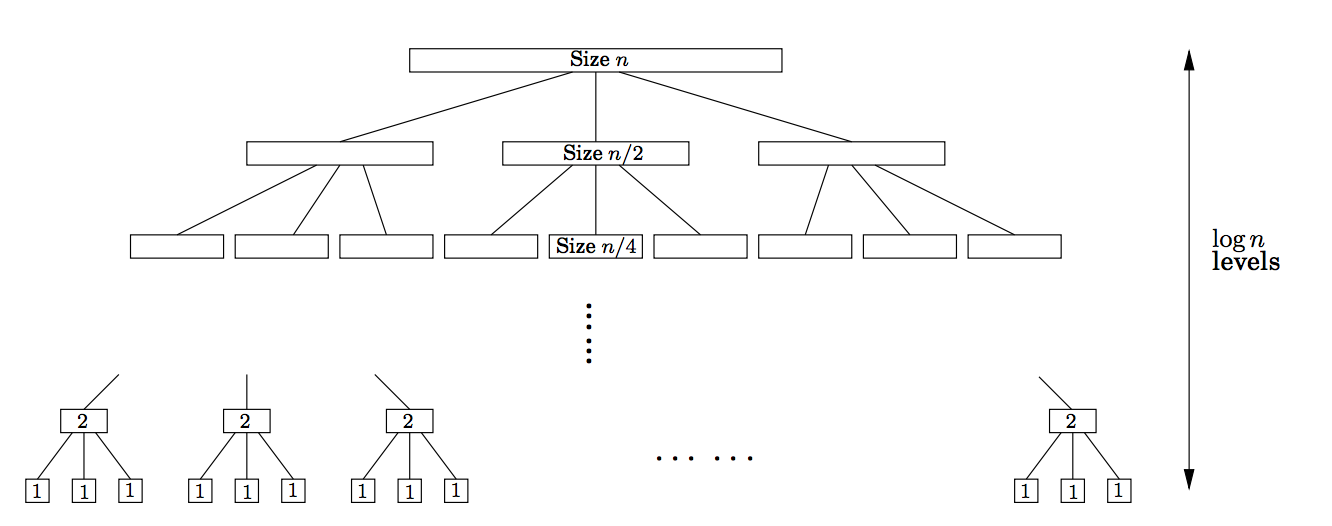
\includegraphics[width=0.3\textwidth]{divide_and_conquer.png}
\caption{\label{fig:divide_and_conquer}Divide and Conquer}
\end{figure}
\item
$O(n^{2})$ - Quadratic\\ 
Eg. Bubble sort, quick sort $\Rightarrow$ Worst:$O(n^{2})$; Average: $O(nlogn)$
\item
$O(n^{3})$ - Cubic time\\ 
Eg. Count the number of triangles in graphs
\item
$O(logn)$\\
Eg. Searching sorted array; Binary Tree Search(Balance Tree)
\end{enumerate}

\pagebreak
\textbf{9.Hash table}
\begin{itemize}
\item 
It is a data structure used to implement an associative array, a structure that can map keys to values. It adopts hash function to compute an index into an array of buckets or slots with values. (Figure5)
\begin{figure}
\centering
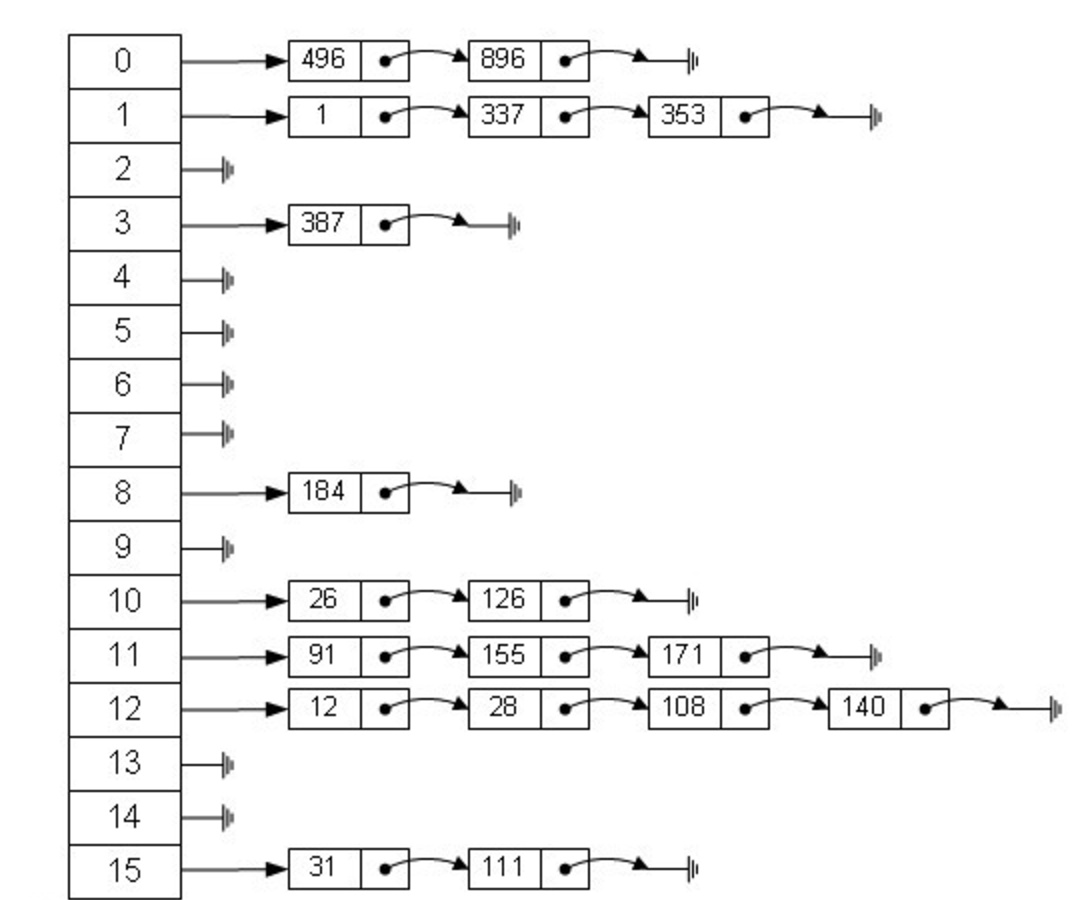
\includegraphics[width=0.3\textwidth]{hash_table.png}
\caption{\label{fig:Hash Table}Hash Table.}
\end{figure}
\item
Hash collisions are unavoidable in practice because hashing a random subset of a large set of possible keys often occurs.
\item
Eg. Query problem:
\begin{itemize}
\item 
Sorting $\Rightarrow$ $O(nlogn)$
\item
Hash Table $\Rightarrow$ $O(n)$
\end{itemize}
\end{itemize}


